\section{Cloud Grading Architecture With OpenEdX}
\label{sec:arch}

We believed the best way to build a robust and scalable autograder was
to adopt a narrow Unix-like view of what an autograder does: it is a
stateless command-line program that, given a student work submission and
a rubric, computes a score and some textual feedback.  We then treat
separately the question of how to connect this program to an LMS.

All other policy issues---whether students can resubmit homeworks, how
late penalties are computes, where the gradebook is stored, any other
LMS behaviors---are out of scope, as is the question of whether these
autograders should replace or supplement manual grading by instructors.

\subsection{OpenEdX and XQueues}

\tbd{point to OpenEdX documentation}

OpenEdX defines a protocol for interacting with so-called ``external
graders.''  When a student using OpenEdX submits an assignment that is
to be graded by an external grader, the student's submitted file goes
into a persistent named queue called an XQueue; each course has its own
XQueue.  OpenEdX exposes a 
authenticated RESTful API \tbd{need citation for RESTful API} through which an
external grader can retrieve a student assignment from an XQueue and
later post back a numerical grade and textual feedback.  
The student submission form can be configured to include additional
metadata for the autograder; we use that field to distinguish different
assignments so that the autograder knows which rubric files must be used.

Retrieving an
assignment and posting back a 
grade are separate queue operations, to allow for autograders that may
take a long time to run.  
If the autograder polls the XQueue and finds it empty, the grader
process sleeps for awhile and tries again.  (In the future we will allow
idle autograders to kill themselves.)
If an assignment is retrieved but no grade is posted back before a
preset timeout, OpenEdX returns the assignment to the queue, where it will
eventually be picked up again by another autograder instance.
Therefore, if an autograder crashes while grading an assignment, no
student work is lost.

This architecture makes it relatively straightforward to absorb a large
burst of assignment submissions: since  the autograders 
  themselves are stateless and the only state is in the XQueues,
we simply deploy additional copies of
the VM instances on Amazon's cloud.  Since grading is embarrassingly
task-parallel, each autograder instance we deploy results in a linear
increase in the rate at which the queue is serviced.  
Even our most sophisticated autograders take less than one
machine-minute per assignment, so at less than 10 cents per machine-hour,
MOOC-scale 
autograding is cost-effective and fast: even with
thousands of assignments being submitted in a 50,000-learner course,
students rarely waited more than a few minutes to get feedback.

OpenEdX also supports an alternative protocol in which each student
submission event triggers a call to a RESTful autograder endpoint,
effectively having OpenEdX ``push'' submissions to the autograder rather
than having the autograder ``pull'' them.  We do not use this
alternative protocol because it would thwart this simple scaling trick
and because we might find ourselves unable to limit the rate at which
submissions were pushed to our autograders.

The external grader does not have access to
the identity of the learner; instead, an obfuscated token identifies the
learner, with the mappings to the learners' true identities maintained only on the
OpenEdX LMS.  Hence no sensitive information connecting a work product
to a specific student is leaked if the autograder is compromised.

\begin{figure}
  \centering
  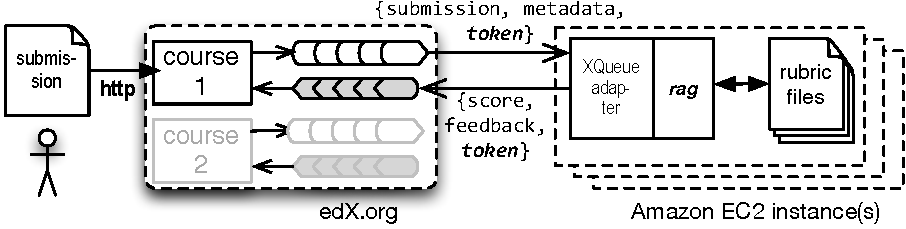
\includegraphics[width=0.75\textwidth]{autograder_arch.pdf}
  \caption{\label{fig:arch}
  Since our autograders rely on many libraries,
  tools, support files, and so on, we encapsulate the autograder in a
  virtual machine image that is deployed on Amazon Elastic Compute Cloud.
  When a new instance is started, the autograder script automatically runs from
  \texttt{/etc/init.d} and examines a deploy-time environment variable
  to get obtain the credentials needed to make calls to the XQueues.}
\end{figure}


\subsection{Rubric Files}

autograder, rubric file

current refactoring to allow rubric files to be pulled on demand and
updated in place

\subsection{CI Workflow for Autograders}

\tbd{Paul to describe CI workflow for ensuring autograders working
  properly}


\begin{figure}
  Cucumber code snippet here from one of the homework's CI files
  \caption{\label{fig:rag-ci}%
Example Cucumber scenario, run in CI, that ensures the autograder works
correctly given a correct submission.
}
\end{figure}


\subsection{Robustness and Security}

Multiple layers of security: watchdog timers, sandboxed interpreter, threads. Hollingsworth 1960 observed that it was possible for students to submit programs that deliberately damage the autograder.

Trustworthiness: because we control the VM image in which the
  autograder runs and the grades are recorded to a central queue server
  which we also control, students cannot tamper with the autograder's
  results or functioning.

Sandboxing: while our RSpec-based autograder performs much of its
  own sandboxing, even if student code escapes the sandbox we can shut
  down and undeploy the VM.  

  TBD Watchdog timers that do this if miss several heartbeats.




